\documentclass{article}
\usepackage{amsmath}
\usepackage{amsthm}
\usepackage{amsfonts}
\usepackage{amssymb}
\usepackage{bbold}
\usepackage{dsfont}
\usepackage{graphicx}
\usepackage{cleveref}
\usepackage{bm}
\usepackage{booktabs}
\usepackage{siunitx}
\usepackage{xcolor}
\usepackage[utf8]{inputenc}
\usepackage[english]{babel}
\newtheorem{definition}{Definition}
\newtheorem{example}{Example}
\newcommand{\exP}[1]{\mathrm{e}^{#1}}
\newcommand{\dif}{\mathrm{d}}
\renewcommand{\vec}[1]{\mathbf{#1}}
\newcommand{\pdagger}{{\phantom{\dagger}}}
\newcommand{\state}[1]{\vert #1\rangle}
\newcommand{\cstate}[1]{\langle #1\vert}
\newcommand{\tr}[1]{\mathrm{tr}\left\{#1\right\}}
\newcommand{\trs}[2]{\, \mathrm{tr}_{#1}\{#2\}}
\newcommand{\expc}[3]{\langle #1\vert #2 \vert #3\rangle}
\usepackage[doi=false,url=false,isbn=false,backend=bibtex,style=nature,natbib=true,sorting=none]{biblatex}
\bibliography{bib.bib}
\usepackage{geometry}
\geometry{
	a4paper,
	total={170mm,257mm},
	left=20mm,
	top=20mm,
}
\begin{document}
	
\title{Report 5: Comparison of TT-HEOM with MF-HEOM. Holstein and Peierls Model}
\author{Rudolf Smorka}
\maketitle
%\tableofcontents
\section{Born-Oppenheimer potential energy of the three-site Fransson model}
The Born-Oppenheimer approximation yields the following Hamiltonian for the three-site Fransson model
\begin{equation}
	H_\mathrm{BO} = \begin{pmatrix}
		\left(\varepsilon_1 + \frac{\omega_0^2 X_1^2}{2}\right) \mathds{1} & -(t_0 +t_1\sqrt{2\omega_0}X_1)\mathds{1} & (\lambda_0 + \lambda_1\sqrt{2\omega_0}X_1)\vec{v}_{13}^{(+)}\cdot\bm{\sigma}\\
		-(t_0 +t_1\sqrt{2\omega_0}X_1)\mathds{1} & \left(\varepsilon_2 + \frac{\omega_0^2 X_2^2}{2}\right) \mathds{1} & -(t_0 +t_1\sqrt{2\omega_0}X_2)\mathds{1} \\
		(\lambda_0 + \lambda_1\sqrt{2\omega_0}X_2)\vec{v}_{31}^{(+)}\cdot\bm{\sigma}&  -(t_0 +t_1\sqrt{2\omega_0}X_2)\mathds{1} & \varepsilon_3 \mathds{1}
	\end{pmatrix}.\label{eq:BO_Hamiltonian_Fransson_1x3}
\end{equation}
The adiabatic potential energy surfaces for various values of $t_1$ and $\lambda_1$ (other parameters are the same as in \cref{sec:1_Comp_TTHEOM_MFHEOM}) are shown in \cref{fig:PES_1x3_lambda1_t1_Var}. Note that the Hamiltonian \cref{eq:BO_Hamiltonian_Fransson_1x3} is 6-dimensional due to the spin of the electron. However, because the spin-orbit coupling $\lambda_0$ is 40 times smaller than $t_0$ and 4 times smaller than $t_1$, the two-fold degeneracy of eigenstates is lifted on an energy-scale much smaller than variations of the energies when varying vibrational displacements. Shown are the influence of $t_1$ alone (a$_1$)-(a$_3$), $\lambda_1$ alone (b$_1$)-(b$_3$), and the case where $t_1=\lambda_1$ (c$_1$)-(c$_3$). Since $\lambda_1=\frac{t_1}{40}$, the BO-potential energy surfaces of the Fransson model investigated in the previous section are very similar to the ones shown in \cref{fig:PES_1x3_lambda1_t1_Var} (a$_1$)-(a$_3$). We denote the states of the purple PES by $S_1,S_2$, the green one by $S_3,S_4$ and the gold one by $S_5,S_6$.
Notable points are the avoided crossings of states $S_1,S_2$ with $S_3,S_4$ at $X_1=-69,-160$ and states $S_3,S_4$ with $S_5,S_6$ at $X_1=-159,-160$. 
\begin{figure}[!h]
	\centering
	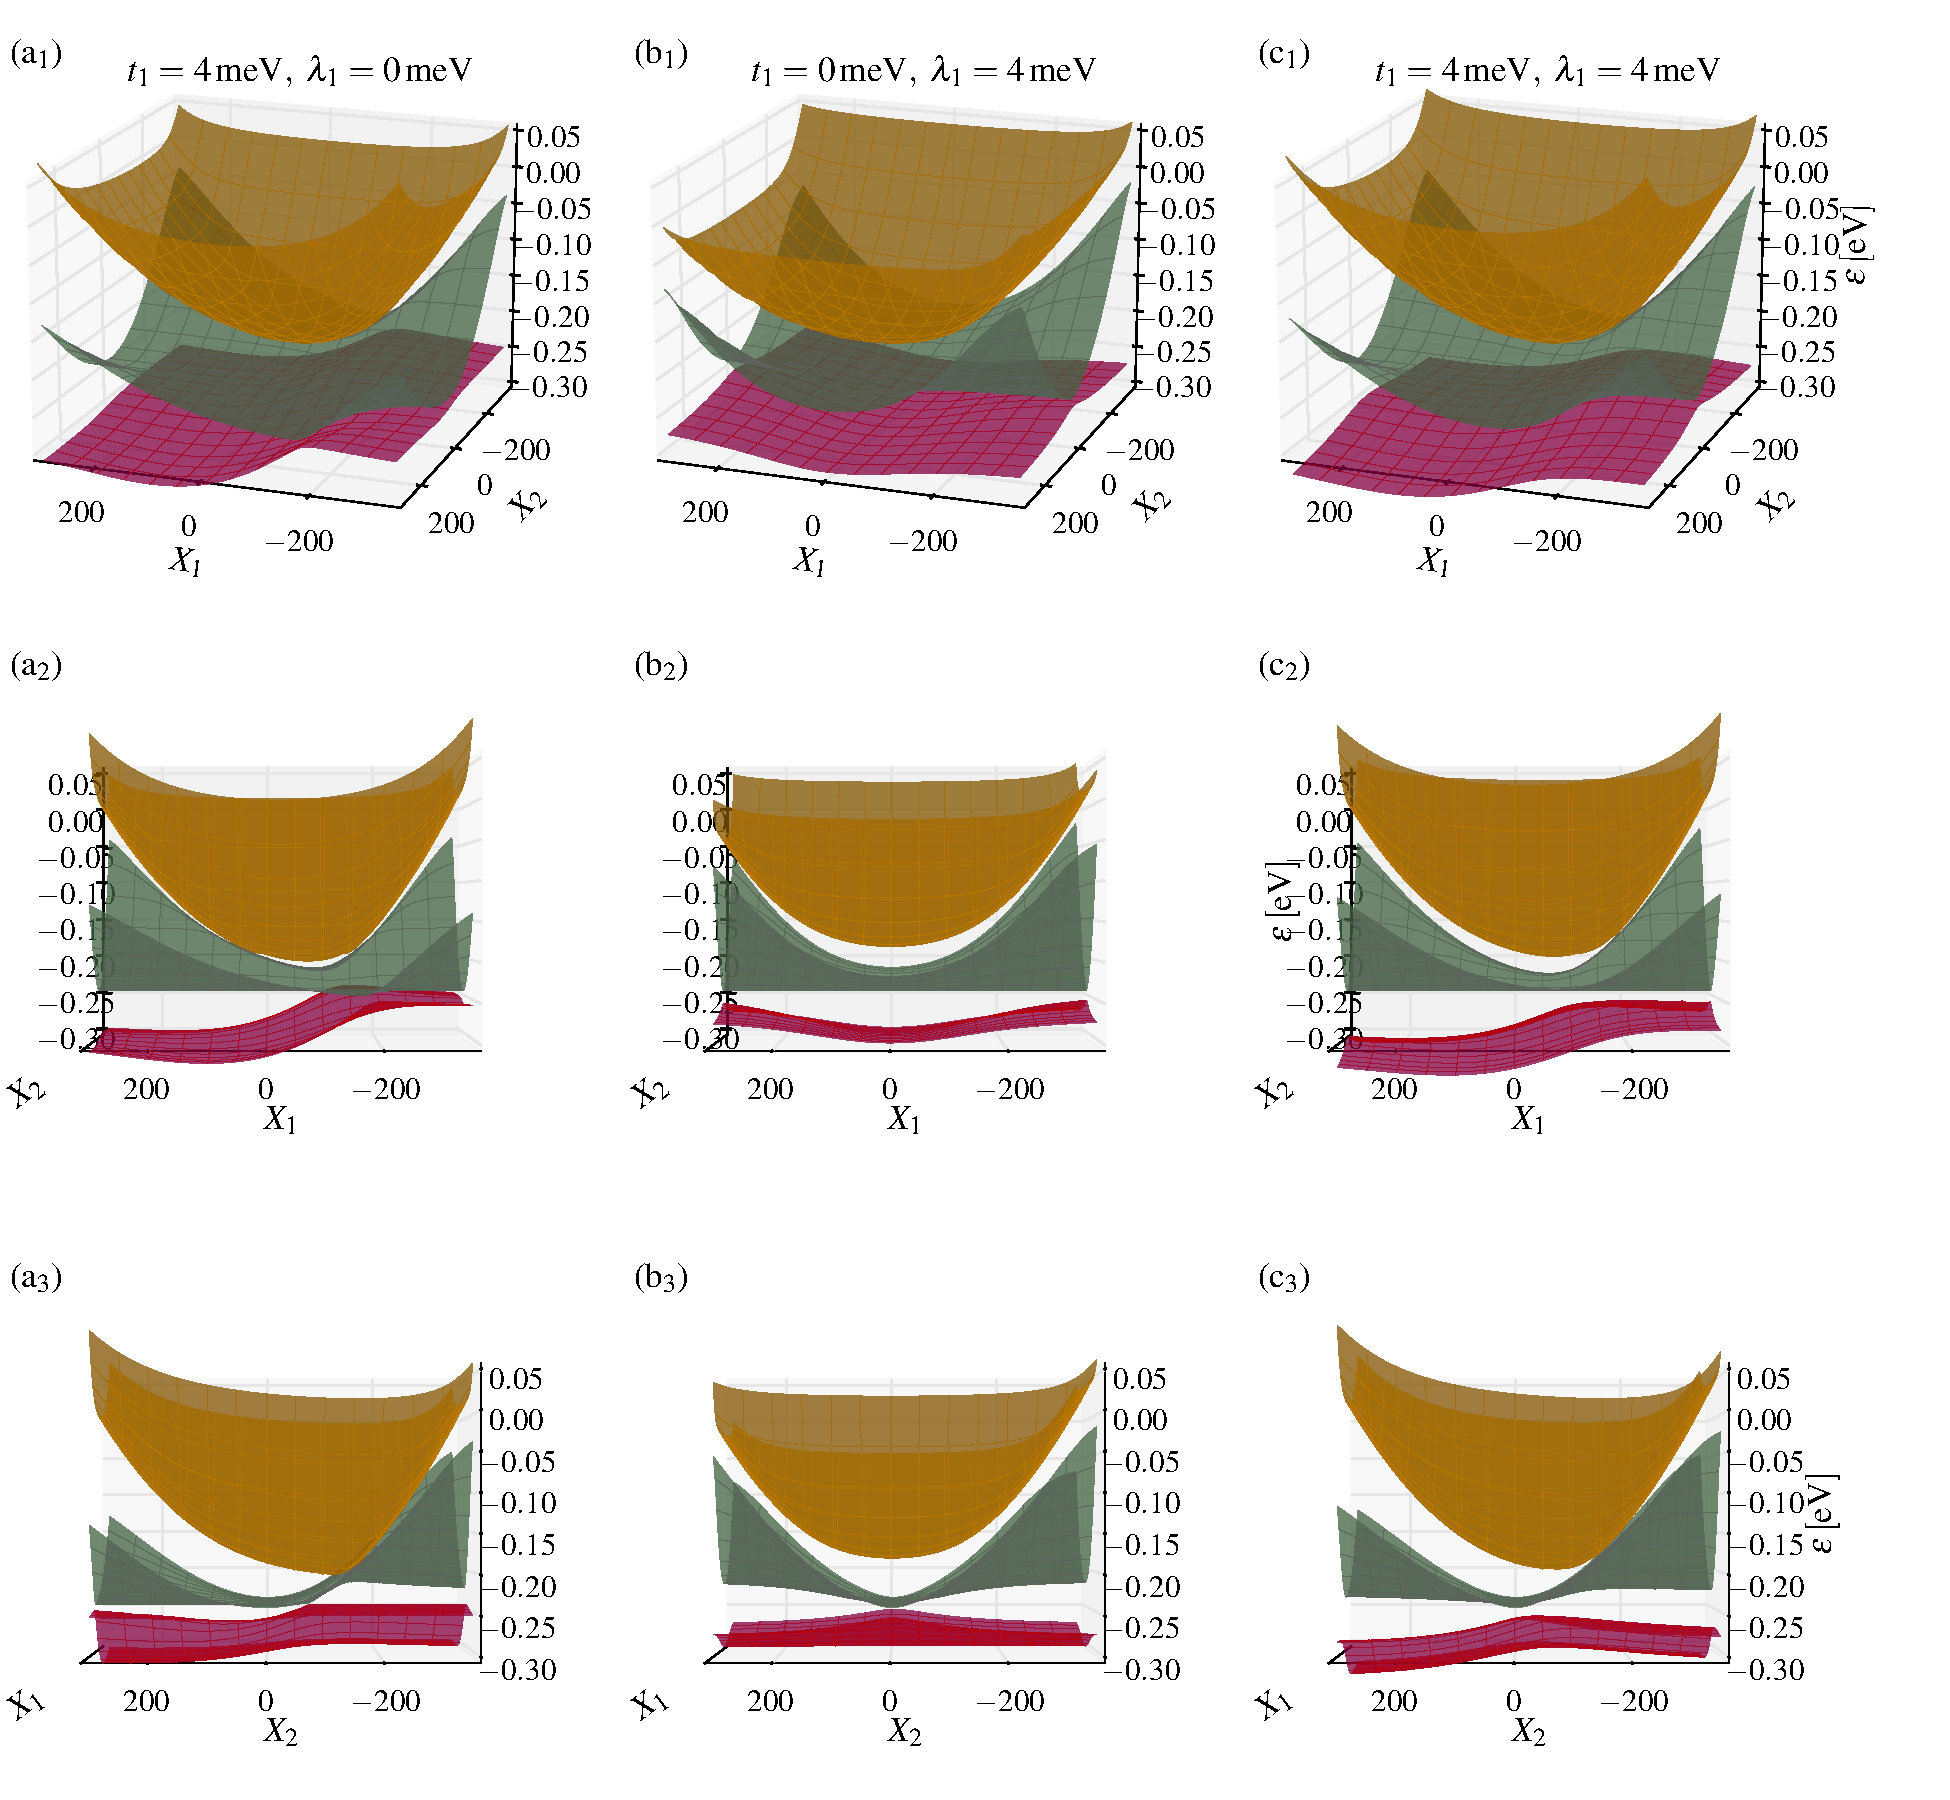
\includegraphics[width=0.99\textwidth]{figs/PES_1x3_SOC0.001_tPh0.004_SOCPh0.0001_multiState_multiAngle.pdf}
	\caption{Adiabatic potential energy surfaces for the Fransson model with molecular size $\mathbb{M}=1\times 3$, $t_0=\SI{40}{\milli\electronvolt}$, $\lambda_0 = \SI{0.1}{\milli\electronvolt}$ and $\omega_0 = \SI{2}{\milli\electronvolt}$ for $t_1=\SI{4}{\milli\electronvolt}$ and $\lambda_1 = \SI{0}{\milli\electronvolt}$ (a$_1$)-(a$_3$), $t_1=\SI{0}{\milli\electronvolt}$ and $\lambda_1 = \SI{4}{\milli\electronvolt}$ (b$_1$)-(b$_3$), and $t_1=\SI{4}{\milli\electronvolt}$ and $\lambda_1 = \SI{4}{\milli\electronvolt}$ (c$_1$)-(c$_3$)}\label{fig:PES_1x3_lambda1_t1_Var}
\end{figure}
\begin{figure}[!h]
	\centering
	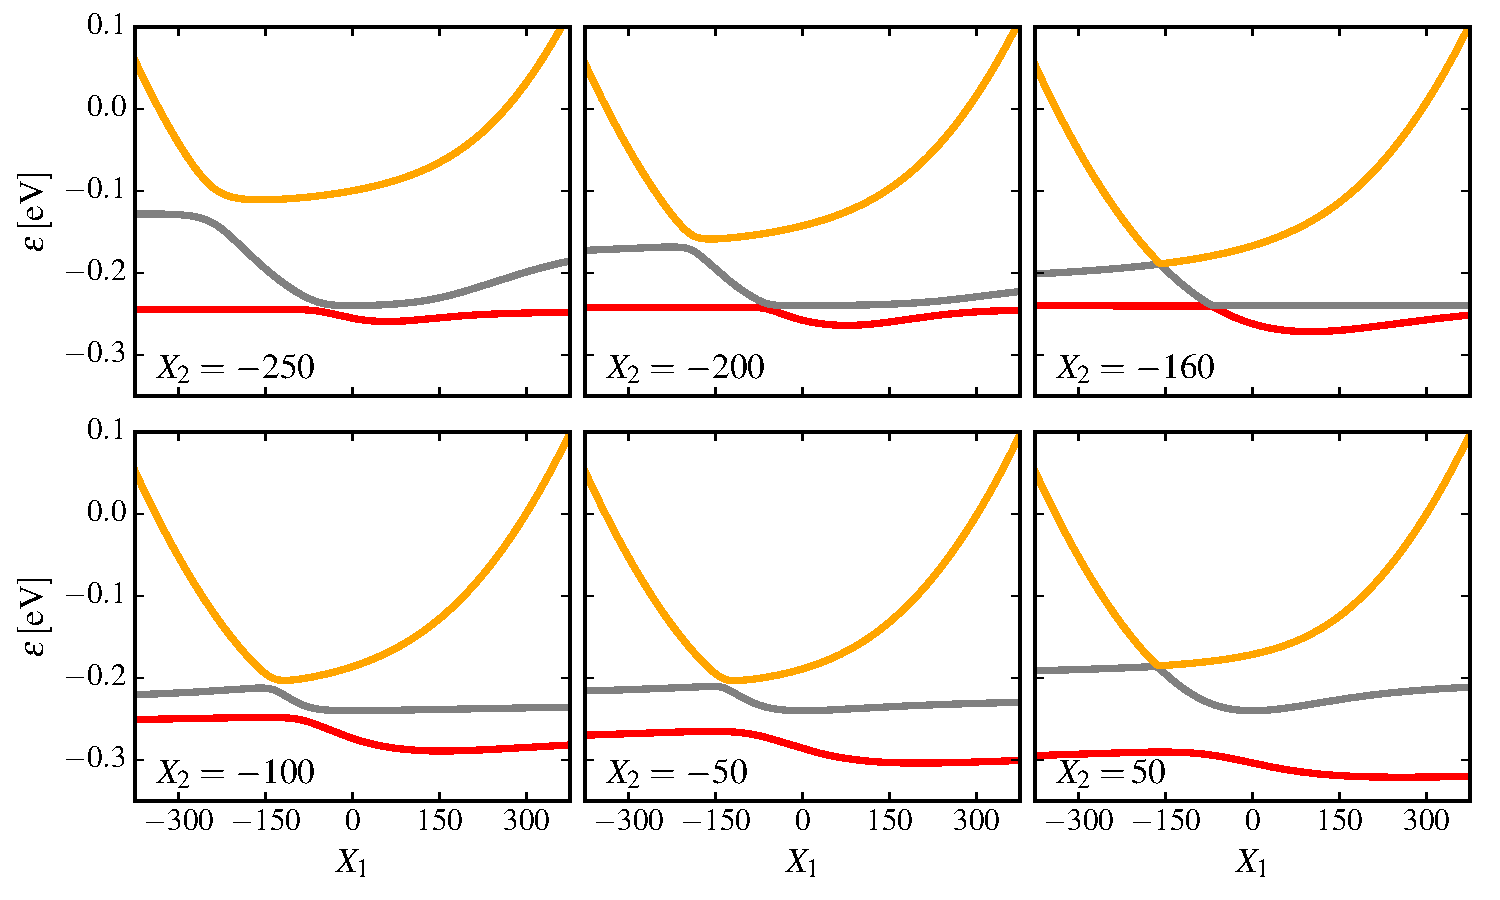
\includegraphics[width=0.99\textwidth]{figs/PES_1x3_SOC0.001_tPh0.004_SOCPh0.0001_multiState_cuts.pdf}
	\caption{BO-states for fixed $X_2$ and varying $X_1$. Parameters are as above.}
\end{figure}
\begin{figure}[!h]
	\centering
	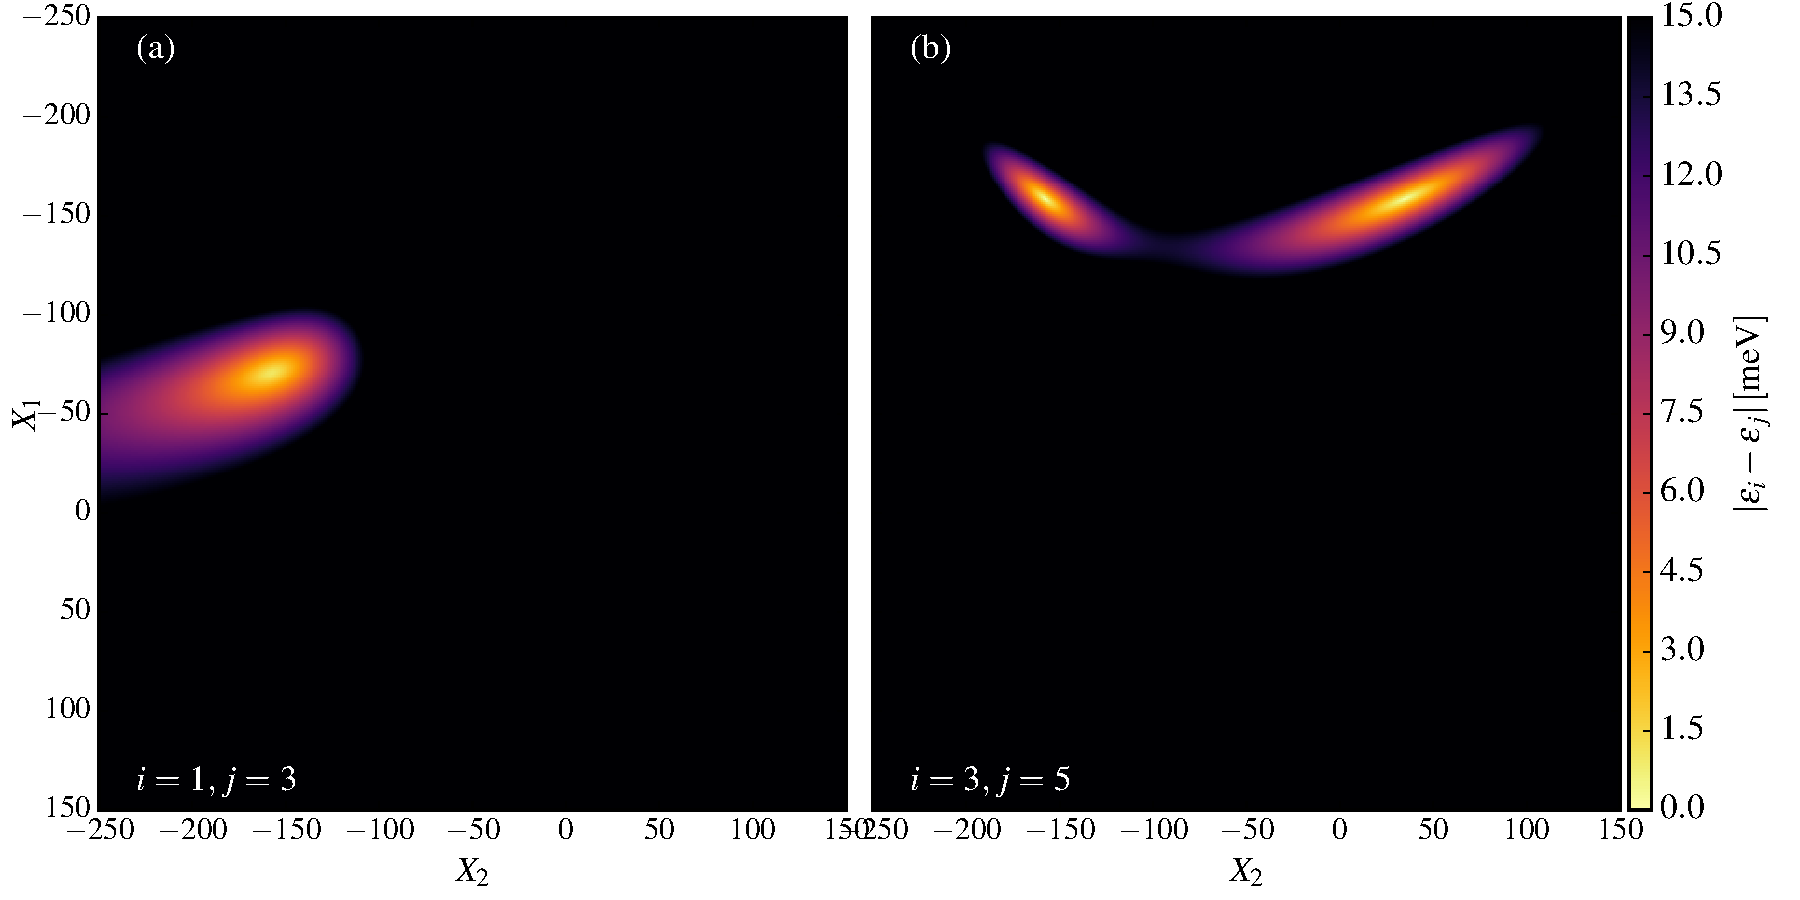
\includegraphics[width=0.99\textwidth]{figs/PES_1x3_SOC0.001_tPh0.004_SOCPh0.0001_multiState_difference.pdf}
	\caption{Absolute difference between BO-eigenstates $S_1$ and $S_3$ (a) and $S_3$ and $S_5$ (b) in the vibrational displacement space.} 
\end{figure}
\clearpage
%\section{Comparison of TT-HEOM with MF-HEOM}\label{sec:1_Comp_TTHEOM_MFHEOM}
%\subsection{Fransson model}
%Parameters: $\mathbb{M}=1\times 3$, $t_0 = \SI{40}{\milli\electronvolt}$, $\lambda_0 = \SI{1}{\milli\electronvolt}$, $t_1=\SI{4}{\milli\electronvolt}$, $\lambda_1 = \SI{0.1}{\milli\electronvolt}$, $\Gamma_0 = \SI{4}{\milli\electronvolt}$ (with lead spin polarization $P = 0.5$), $V=\SI{0.48}{\volt}$ and $T =\SI{ 300}{K}$.
%The following vibrational frequencies are investigated: $\omega_0 = \SI{2}{\milli\electronvolt}$ and $\omega_0=\SI{120}{\milli\electronvolt}$.  
%
%We start with the case low vibrational frequency first, shown in \cref{fig:TTHEOM_MFHEOM_comp_w0_0.05}. There we plot the symmetrized current (a) and the spin-down population on the first site (b), comparing the MF-HEOM results (weighted average over $n=9000$ trajectories sampled from the thermal Wigner distribution for a harmonic oscillator) with TT-HEOM results (various ranks $r$ and number of vibrational states $n_\mathrm{vib}$ for each vibrational mode). Even a rank of $r=200$ and $n_\mathrm{vib}=30$ vibrational states are not sufficient for converging the TT-HEOM results. Although the symmetrized current seems to be converged with increasing the rank and the number of vibrational states in the time-interval until $\sim\SI{5}{\femto\second}$, the population rises above one for all investigated ranks. The unphysical population is obtained already in the first time-step of the calculation.
%\begin{figure}
%	\centering
%	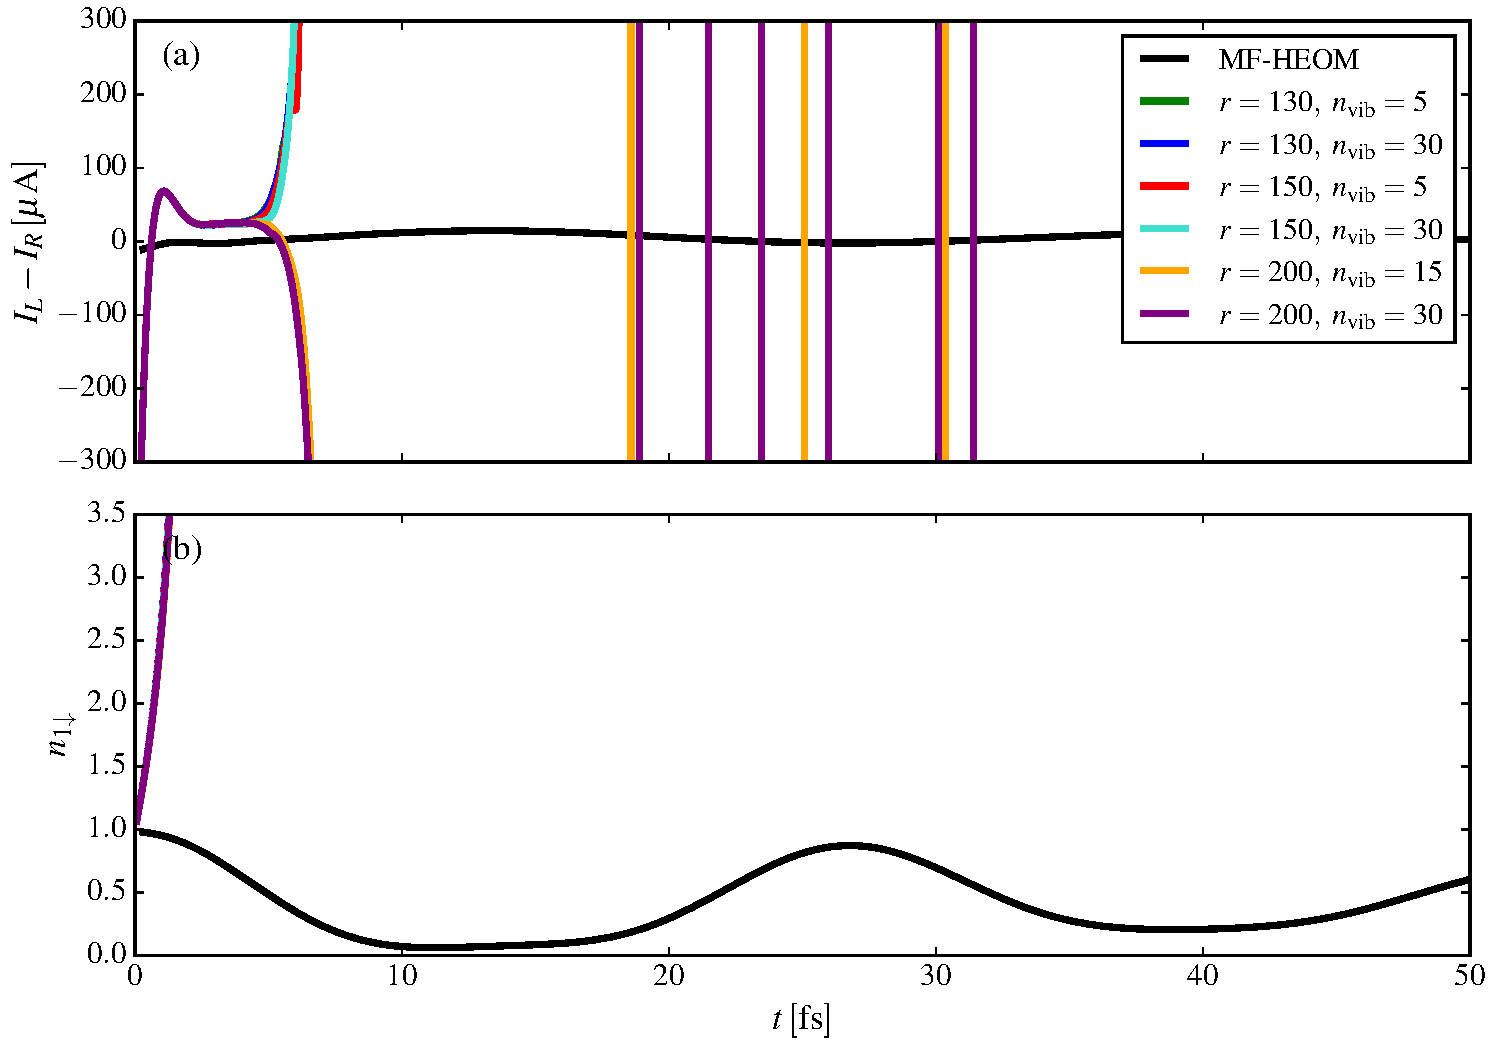
\includegraphics[width=0.9\textwidth]{figs/Comparison_TTHEOM_MFHEOM_1x3_w0_0.05_Gamma0.1t0.pdf}
%	\caption{Comparison of MF-HEOM (sample size $n=9000$) with TT-HEOM (for various rank $r$ and number of vibrational states $n_\mathrm{vib}$): Symmetrized current (a) and population of spin-down electron on the first site (b) for $\omega_0 = \SI{2}{\milli\electronvolt}$. }\label{fig:TTHEOM_MFHEOM_comp_w0_0.05}
%\end{figure}
%
%We now turn to the case with higher vibrational frequency $\omega_0=\SI{120}{\milli\electronvolt}$, shown in \cref{fig:TTHEOM_MFHEOM_comp_w0_3}. In essence, the time-scale on which the symmetrized current and the population diverges within the TT-HEOM, does not significantly change upon increasing the vibrational frequency.
%\begin{figure}
%	\centering
%	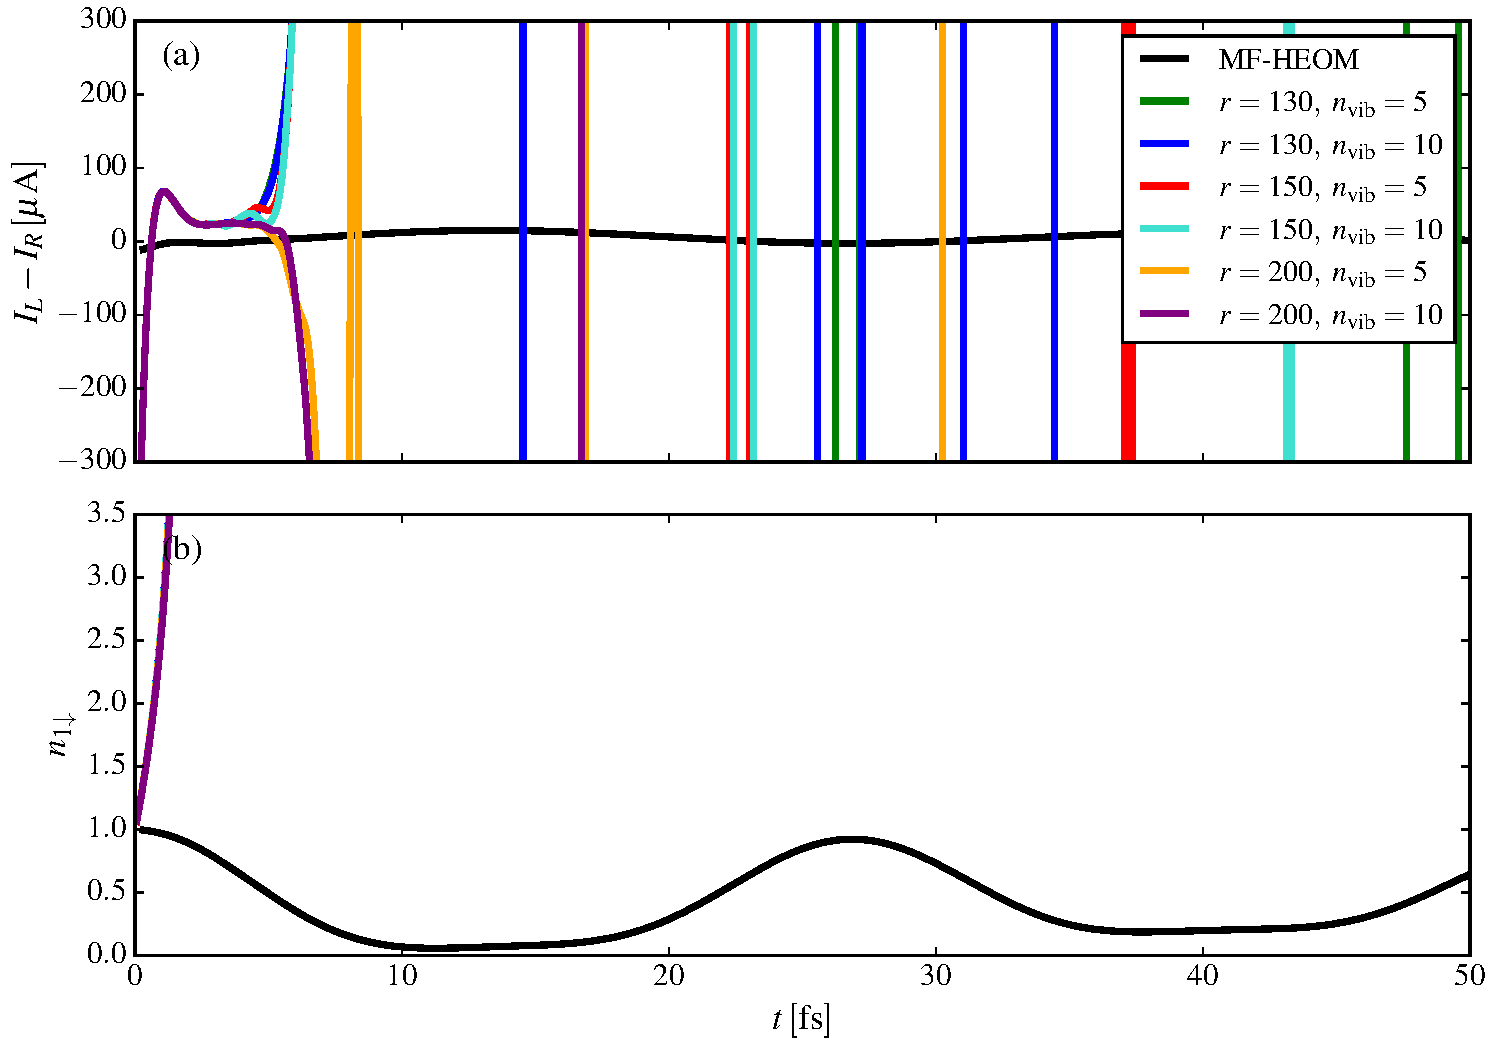
\includegraphics[width=0.9\textwidth]{figs/Comparison_TTHEOM_MFHEOM_1x3_w0_3.0_Gamma0.1t0.pdf}
%	\caption{Same as \cref{fig:TTHEOM_MFHEOM_comp_w0_0.05} for $\omega_0 = \SI{3}{\milli\electronvolt}$. }\label{fig:TTHEOM_MFHEOM_comp_w0_3}
%\end{figure}
\section{Ground State of the Fransson model}
\subsection{Influence of on-site potential}
In the limit of $\varepsilon\rightarrow-\infty$ the ground state of the Fransson model is a product state of doubly occupied electronic sites and all vibrational modes in their lowest energy state
\begin{equation}
	\vert \Psi_\mathrm{GS}\rangle = \vert \uparrow\downarrow,\uparrow\downarrow,\dots,\uparrow\downarrow\rangle\vert 0,\dots,0\rangle.
\end{equation}
\subsection{Influence of Hopping}
Hopping tends to delocalize electrons and due to its off-diagonal contribution the ground state is a superposition over many configurations. The dominant one is with half filling with one electron per site. Contributions with smaller weight are ones in which a single site is doubly occupied and one is empty, while all others are singly occupied. The table below shows representative configurations for $t_0 = \SI{40}{\electronvolt}$ and $\varepsilon = \SI{0}{\electronvolt}$ for $L=6$ (due to spin-flip and translational symmetry of the model in this limit, many configurations are degenerate).
\begin{center}
\begin{tabular}{cc}
	Configuration & Weight\\
	\hline
	$\vert \uparrow,\downarrow,\uparrow,\downarrow,\uparrow,\downarrow\rangle $&  0.1250\\
	$\vert \downarrow,\uparrow\downarrow,0,\uparrow,\downarrow,\uparrow\rangle $&  0.0833\\
	$\vert \uparrow\downarrow,0,\uparrow,\uparrow\downarrow,\downarrow,0\rangle $&  0.0555\\
	$\vert \uparrow,\downarrow,\uparrow\downarrow,\downarrow,\uparrow,0\rangle $&  0.0416\\
	$\vert \uparrow\downarrow,0,\uparrow,\uparrow,\downarrow,\downarrow\rangle $&  0.0277\\
	$\vert \uparrow\downarrow,0,\uparrow\downarrow,0,\uparrow\downarrow,0\rangle$&  -0.1250\\
	\hline
\end{tabular}
\end{center}
\subsection{Influence of SOC}

\end{document}




